% Preamble
\documentclass[12pt,a4paper]{article}
\usepackage{enumerate} 	
\usepackage{setspace}						
\usepackage{authblk}	
\usepackage{graphicx} 	
\usepackage[nomarkers, nolists, figuresonly]{endfloat} 
\usepackage{pdflscape}	
\usepackage{mathtools}	
\usepackage[osf]{mathpazo} 
\usepackage{lineno} 
\usepackage{ms}    	
\usepackage{hyperref}
\usepackage[round]{natbib} 
\usepackage{setspace}

\setcounter{secnumdepth}{0} 
\raggedright 			
\pagenumbering{arabic}	
\linenumbers

% First order headings upper case bold
\usepackage{titlesec}
\titleformat*{\section}{\small\bfseries\uppercase}

% Second order headings normal case italics
\titleformat*{\subsection}{\small\itshape}

% Third order, italics, paragraph style
\titleformat*{\paragraph}{\small\itshape}

% Title page information

\title{Time for a rethink: time sub-sampling methods in disparity-through-time analyses}

\author{
	Thomas Guillerme$^{1}$ and Natalie Cooper$^{2*}$
}

\date{}

\affiliation{\noindent{\footnotesize
	$^1$School of Biological Sciences, University of Queensland, St. Lucia, Queensland, Australia.\\
	$^2$Department of Life Sciences, Natural History Museum, Cromwell Road, London, SW7 5BD, UK. natalie.cooper@nhm.ac.uk}\\
	$^*$Corresponding author\\}

\vfill

\runninghead{Time sub-samples in disparity-through-time analyses}
\keywords{time bin, time-slice, disparity, sub-sampling} 
% up to 6

\begin{document}

\mstitlepage
\parindent = 1.5em
\addtolength{\parskip}{.3em}

\section{Abstract}
% 300 words max

Disparity-through-time analyses can be used to determine how morphological diversity changes in response to mass extinctions, and to investigate the drivers of morphological change.
These analyses are routinely applied to palaeobiological datasets, yet although there is much discussion about how to best calculate disparity, there has been little consideration of how taxa should be sub-sampled through time.
Standard practice is to group taxa into discrete time bins, often based on stratigraphic periods. 
However, this can introduce biases when bins are of unequal size, and implicitly assumes a punctuated model of evolution. 
In addition, many time bins may have few or no taxa, meaning that disparity cannot be calculated for the bin and making it harder to complete downstream analyses.
Here we describe a different method to complement the disparity-through-time tool-kit: time-slicing.
This method uses a time-calibrated phylogenetic tree to sample disparity-through-time at any fixed point in time rather than binning taxa.
It uses all available data (tips, nodes and branches) to increase the power of the analyses, specifies the implied model of evolution (punctuated or gradual), and is implemented in \texttt{R}.
We test the time-slicing method on four example datasets and compare its performance in common disparity-through-time analyses.
We find that the way you time sub-sample your taxa can change your interpretations of the results of disparity-through-time analyses.
We advise using multiple methods for time sub-sampling taxa, rather than just time binning, to gain a better understanding disparity-through-time.

\newpage
\raggedright
\doublespacing
\setlength{\parindent}{1cm}

\section{Introduction}
Disparity-through-time analyses are common in palaeontology \citep{gould1991disparity,briggs1992morphological,Wills1994,Foote01071994}.
They reveal how the morphological diversity of clades has changed through time, and allow us to make inferences about the breadth of ecological niches extinct taxa occupied \citep{foote1997evolution}.
Results from disparity-through-time studies also provide insights into the ecological impacts of mass extinctions, competitive replacements, and the drivers of morphological evolution \citep{Brusatte12092008,Foote29111996,friedmanexplosive2010}.
Unfortunately, the way we perform these analyses may have profound effects on our conclusions.

Disparity-through-time analyses have two main analysis components: calculating disparity, and creating time sub-subsets of the data. 
Here we focus on the latter.
The nature of disparity (i.e. it is a diversity metric), means it cannot be calculated using a single individual, so some way of sub-sampling taxa is required.
Changes in disparity-through-time are generally investigated by calculating the disparity of taxa present during specific time intervals or time bins \citep[e.g][]{cisneros2010,prentice2011,Hughes20082013,hopkinsdecoupling2013,bentonmodels2014,bensonfaunal2014}.
These time bins are usually defined based on stratigraphy \citep[e.g.][]{cisneros2010,prentice2011,Hughes20082013,bentonmodels2014} but can also be arbitrarily chosen time bins of equal (or approximately equal) duration \citep{Butler2012,hopkinsdecoupling2013,bensonfaunal2014}.
However, this approach has several limitations.

First, time bins defined by stratigraphy are not of equal size, biasing higher disparity towards longer stratigraphic periods. 
This can be dealt with using rarefaction methods, i.e. repeating the analysis while resampling the taxa to have the same number of taxa in each bin (e.g. using bootstrapping with limited resampling).
This can, however, lead to large confidence intervals when there are stratigraphic periods with few species.
Other studies split large time bins so they are of roughly equal size, but this is often an \textit{ad hoc} procedure that can introduce more bias depending on where bins are split.
Second, all time binning approaches (whether bins are equally sized or not) assume that characters of taxa evolve following a punctuated equilibrium model, because disparity is only estimated once for each interval resulting in all changes in disparity occurring \textit{between} intervals, rather than also allowing for gradual changes \textit{within} intervals \citep[a pattern that is fairly common in the fossil record;][]{Hunt21042015}.
Third, when investigating changes in disparity due to events at a specific time point (e.g. a mass extinction), time bins may have not have high enough resolution to resolve changes at the event, for example if time bins are every 20 million years it may be hard to capture the effects of an event five million years into the bin.
Finally, time bin analyses are often limited by the number of taxa in each bin.
If there are insufficient taxa in a time bin, disparity cannot be calculated, so further analyses, e.g. correlations of disparity with hypothesised drivers of morphological evolution, are not possible.

To address these issues, we propose a ``time-slicing'' approach that takes advantage of the wealth of palaeontological datasets which now have associated phylogenies. 
Time-slicing uses a phylogenetic tree and considers subsets of taxa at specific equidistant points in time, as opposed to considering subsets of taxa between two points in time (a similar approach is outlined in \citep{halliday2016eutherian}).
This results in even-sampling across time and permits us to define the underlying model of character evolution (punctuated or gradual).  
Time-slicing also includes any element present in the phylogeny (branches, nodes and tips) at the time-slice in question as part of the disparity calculation.
This allows us to measure disparity at time points where there are no sampled terminal taxa, and increases the sample size at each time point, making downstream analyses of the drivers of disparity much more feasible.

Here we present our time-slicing methods using four datasets taken from the literature.
We calculate disparity-through-time for each dataset using a range of time binning and time-slicing methods, and then compare these approaches with respect to the relative disparities calculated, but also investigate how the different approaches influence biological conclusions. 
We find that the choice of time sub-sampling method can have profound effects on the conclusions of disparity-through-time analyses. 

\section{Materials and Methods}
\subsection{Overview}
\label{overview-section}
To test the different time sub-sampling methods, we followed the protocol below (Fig. \ref{fig:overview}). 
All the code needed to reproduce these analyses (along with detailed instructions) is provided on GitHub (\url{https://github.com/nhcooper123/time-slice}.
% NC: Add proper reference to this before publication.

% overview figure
\begin{figure}[!htbp]
    \centering
    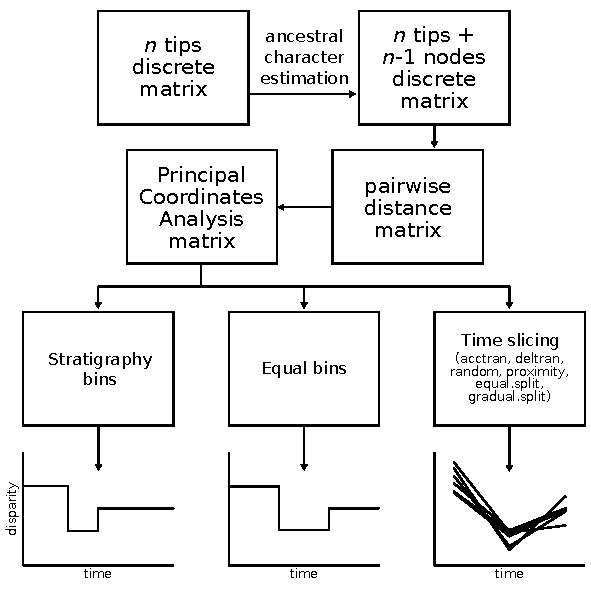
\includegraphics[width=1\linewidth, height=1\textheight, keepaspectratio]{figures/Figure1-outlinesvg.pdf}
    \caption[Outline of the disparity-through-time pipeline]
    {Outline of the disparity-through-time pipeline. 1) We use ancestral character estimation to infer nodal character states; 2) we measure the pairwise Gower distance between the tip character states and nodal character states; 3) we ordinate the distance matrix using principal coordinates analysis (PCoA); 4) we time sub-sample the PCoA matrix using time bins defined by stratigraphic periods, equally sized time bins and time-slices (using six methods to estimate ordination scores for branches); and finally 5) we measure disparity-through-time for each of these methods.}
    \label{fig:overview}
\end{figure}

\subsection{Example datasets}
\label{datasets}
To test the different time binning/slicing methods we selected four datasets: a mammal dataset from \cite{beckancient2014}, two theropod datasets from \cite{brusatte2014gradual} and \cite{bapst2016topology}, and a crinoid dataset from \cite{wright2017bayesian}.
Table \ref{table:datasets} and the Supporting Information Appendix S1 provide more details. 
Each dataset consists of first and last occurrence dates for all taxa, a matrix of morphological characters in NEXUS format, and a time-scaled phylogeny. 
These datasets are freely available with their accompanying papers (Table \ref{table:datasets}), but for reproducibility purposes we also provide the data we used on GitHub (\url{https://github.com/nhcooper123/time-slice/data}).

% Dataset details table
%\begin{landscape}
%% latex table generated in R 3.4.3 by xtable 1.8-2 package
% Wed Dec 20 13:12:18 2017
\begin{table}[!htbp]
\caption{Details of the datasets used in this study. Age ranges are root time to most recent tip taxon.} 
\centering
\begin{tabular}{lcccc}
  \hline
 & \textbf{Beck2014} & \textbf{Brusatte2014} & \textbf{Bapst2016} & \textbf{Wright2017} \\ 
  \hline
Group & mammals & theropods & theropods & crinoids \\ 
  \# taxa & 106 & 152 &  89 &  42 \\ 
  \# characters & 421 & 853 & 374 &  87 \\ 
  Age range (MYA) & 171.8 - 0 & 168.5 - 66 & 207.2 - 66 & 485.4 - 372.2 \\ 
  Mass extinction (MYA) & 66 (K-Pg) & NA & NA & 443 (O-S) \\ 
  Reference & \cite{beckancient2014} & \cite{brusatte2014gradual} & \cite{bapst2016topology} & \cite{wright2017bayesian} \\ 
  Data reference &  \cite{beckancient2014} & \cite{dryad_84t75} & \cite{dryad_n2g80} &  \cite{dryad_6hb7j} \\ 
   \hline
\end{tabular}
\label{table:datasets}  
\end{table}
 
  % Label in input or referencing doesn't work
%\end{landscape}

\subsection{Preparing the data for disparity-through-time analysis}

\paragraph{Estimating ancestral character states.}
\label{ace}
For each dataset we estimated the ancestral character states at each node using the \texttt{AncStatesEstMatrix} function from the \texttt{Claddis} \texttt{R} package \citep{Claddis,R}.
This function uses the re-rooting method \citep{Yang01121995,Garland2000} to get Maximum Likelihood estimates of the ancestral states for each character at every node in the phylogeny \citep[based on the \texttt{rerootingMethod} function in \texttt{phytools};][]{phytools}.
Inapplicable and missing characters for any taxon were treated as ambiguous characters (i.e. any possible observed state for the character).
% NC: I've left this one bit to make it clear but removed the explanation (this was all just copied from your thesis)
To prevent poor ancestral state estimations from biasing our results, especially when a lot of error is associated with the estimations, we only included ancestral state estimations with a scaled Likelihood $\geq$ $0.95$.
Ancestral state estimations with scaled Likelihoods below this threshold were recoded as missing data (``?'').
This allowed our results to be less dependent on the quality (or the absence thereof) of the ancestral state estimations methods, especially in parts of the datasets where data were sparse. 
This approach is similar to \cite{brusatte2011phylogenetic} but uses model based estimations (rather than parsimony) allowing to control for ambiguous nodes (i.e. poorly estimated).

\paragraph{Building morphospaces.} 
% To explore disparity-through-time in our datasets we used a morphospace approach \citep[e.g.][]{Foote01071994,Foote29111996,Wesley-Hunt2005,Brusatte12092008,friedmanexplosive2010,toljagictriassic-jurassic2013,Hughes20082013}.
% This approach is similar to constructing a morphospace based on continuous morphological data \citep[e.g.][]{friedmanexplosive2010}, except a morphospace is an approximation of the morphospace based on discrete morphological data (i.e. the discrete morphological characters used to build a phylogenetic tree, often referred to as ``cladistic'' data).
% %TG: about that, I'm actually less and less convinced we should call it caldisto-space: first, semantically, cladistic data means data used to make clades (phylos) so it could be nucleotides as well. Second, during the PhD, we used morphospace to distinguish it from the morpho-space but at that time I was naively thinking the the morpho-space is the morphometric-space (which it often is!) but, again, semantically, the morpho-space can also be simply the morphology-space... However, I like the sound of morphospace and most people will understand it the way we do. I'm just thinking about pedantic-palaeo-reviewers...
% % NC: Good point. Let's leave it for now as I think this bit is nicely explained, but easy enough to edit if people don't like it.
% Mathematically, a morphospace is an $n$ dimensional object that summarises the cladistic distances between the taxa present in a cladistic matrix.
% Although empirically inter-taxon distances are the same in a morphospace or a morphospace \citep{foth2012different,hetherington2015cladistic}, we prefer the term morphospace to make it clear that this space is estimated using cladistic data and not morphometric data.



To explore disparity-through-time in our datasets, we used a morphospace approach \citep[e.g.][]{Foote01071994,Foote29111996,Wesley-Hunt2005,Brusatte12092008,friedmanexplosive2010,toljagictriassic-jurassic2013,Hughes20082013}.
Morphospace can be obtained from any multidimensional morphological data set but can differ in the data used (e.g. discrete or continuous) or whether they include phylogenetic data or not.
Although empirical morphospaces from discrete or continuous data have been shown to have similar properties \citep{foth2012different,hetherington2015cladistic}, we would like to highlight that our morphospaces are based on discrete morphological data (originally collected for phylogenetic analysis; \textit{c.f.} geometric morphometric data) and includes some phylogenetic information (see above).
Mathematically, our morphospaces are $n$ dimensional objects that summarises the distances between discrete morphological characters of the taxa present and their ancestors.


\paragraph{Constructing distance matrices.}
To estimate the morphospaces for each of our datasets we first constructed pairwise distance matrices of length $k$, where $k$ is the total number of tips and nodes in the dataset.
We calculated the $k$$\times$$k$ distances using the Gower distance \citep{Gower71}, i.e. the Euclidean distance between two taxa divided by the number of shared characters. 
This allows us to correct for distances between two taxa that share many characters and could be closer to each other than to taxa with fewer characters in common (i.e. because some pairs of taxa share more characters in common than others, they are more likely to be similar).
For discrete morphological matrices, using this corrected distance is preferable to the raw Euclidean distance because of its ability to deal with discrete or/and ordinated characters as well as with missing data \citep{anderson2012using}.
However, the Gower distance cannot calculate distances when taxa have no overlapping data.
Therefore, we used the \texttt{TrimMorphDistMatrix} function from the \texttt{Claddis} \texttt{R} package to remove pairs of taxa with no cladistic characters in common.
This led to us removing nine taxa from the \cite{bapst2016topology} dataset, and 19 from the \cite{brusatte2014gradual} dataset, but none from the other two datasets (see Supporting Information Appendix S1 for details of which species). 

\paragraph{Ordination.}
After constructing our distance matrices we transformed them using classical multidimensional scaling \citep[MDS;][]{torgerson1965multidimensional,GOWER01121966,cailliez1983analytical}.
This method (also referred to as PCO; e.g. \citealt{Brusatte2015}; or PCoA; e.g. \citealt{paradisape:2004}; but distinguished in \citealt{legendre2012numerical}) is an eigen decomposition of the distance matrix.
Because we used Gower distances instead of raw Euclidean distances, negative eigenvalues can be calculated.
To avoid this problem, we first transformed the distance matrices by applying the Cailliez correction \citep{cailliez1983analytical} which adds a constant $c^*$ to the values in a distance matrix (apart from the diagonal) so that all the Gower distances become Euclidean ($d_{Gower}+c^*=d_{Euclidean}$; \citealt{cailliez1983analytical}). 
We were then able to extract $n$ eigenvectors for each matrix (representing the $n$ dimensions of the morphospace) where $n$ is equal to $k-2$, i.e. the number of taxa in the matrix ($k$) minus the last two eigenvectors that are always null after applying the Cailliez correction.
Contrary to previous studies \citep[e.g][]{brusatte50,cisneros2010,prentice2011,anderson2012using,Hughes20082013,bentonmodels2014}, we use all $n$ dimensions of our morphospaces and not a sub-sample representing the majority of the variance in the distance matrix (e.g. selecting only $m$ dimensions that represent up to 90\% of the variance in the distance matrix; \citealt{Brusatte12092008,toljagictriassic-jurassic2013}).

Note that our morphospaces represent an ordination of all possible morphologies coded in each study through time.
It is unlikely that all morphologies will co-occur at each time point, therefore, the disparity of the whole morphospace is expected to be greater than the disparity at any specific point in time.

\subsection{Disparity-through-time analyses}

Disparity-through-time analyses were performed using the \texttt{dispRity} \texttt{R} package \citep{dispRity.v02}. 
% NC: Update reference here prior to publication

\paragraph{Calculating disparity.}
\label{disparity_calc}
Disparity can be calculated in many different ways \citep[e.g.][]{Wills1994,Ciampaglio2004,thorneresetting2011,hopkinsdecoupling2013,huang2015origins}, however a majority of studies in palaeobiology estimate disparity using four metrics: the sum and products of ranges and variances, each of which gives a slightly different estimate of how the data fits within the morphospace \citep{Foote01071994,Wills1994,brusatte50,Brusatte12092008,cisneros2010,thorneresetting2011,prentice2011,brusattedinosaur2012,toljagictriassic-jurassic2013,ruta2013,bentonmodels2014,bensonfaunal2014}.
However, these metrics have limitations. 
First, the range metrics are affected by the uneven sampling of the fossil record \citep{Butler2012}.
Second, because we include all $n$ dimensions in the analysis (see above), the products of ranges and variances will tend towards zero since the scores of the last dimension are usually really close to zero themselves. 
We therefore use the sum of variances metric to estimate disparity here:

\begin{equation}
\text{disparity} = \sum\sigma^{2}{n_i}
\end{equation}

Where $\sigma^{2}{n_i}$ is the variance for the $n_i^{th}$ dimension ranging from $k$ to $k-2$ with $k$ being the number of taxa in the dataset.
Note that there are still statistical issues with this metric (such as the co-variance between dimensions not being measured), but for the purposes of comparison with previous work we decided to use a standard metric for these analyses.

\paragraph{Time sub-sampling} 
\label{time_sub-samples}

To estimate disparity-through-time we first need to split the data into time sub-samples.
Here we use three time sub-sampling methods.

\begin{enumerate}
  \item Stratigraphic time bins. This is the traditional method, where all the taxa within each stratigraphic period are included in the disparity calculation. This often leads to bins of unequal duration. Here we use stratigraphic stages and epochs.
  \item Equally sized time bins. This is another commonly used method, where the time frame of interest is split into equally sized time bins, then all the taxa within each time bin are included in the disparity calculation. 
  \item Time-slicing. We describe this in more detail below, but in brief, time-slicing uses a phylogeny, and rather than binning the data, it takes slices through a phylogeny and includes all the taxa and nodes in that slice within the disparity calculation. 
\end{enumerate}  

\paragraph{Time-slicing.} 
\label{time_slicing}
The ``time-slicing'' approach considers subsets of taxa in the morphospace at specific equidistant points in time, as opposed to considering subsets of taxa between two points in time.
This results in even-sampling of the morphospace across time and allows us to use different underlying models of character evolution (punctuated or gradual). 

%TG: Is it worth saying that Halliday and Goswami came up with a similar idea \citep{halliday2016eutherian} but that we came up with it first \cite{Guillerme2015} and we're the first to implement it \cite{dispRity.v02}?
%NC: Yeah was going to ask about this - I've added a mention to the intro where I think it fits better, should we also cite the brusatte paper you said refers to it too?

In practice, time-slicing considers the disparity of any element present in the phylogeny (branches, nodes and tips) at any point in time.
When the phylogenetic elements are nodes or tips, the ordination scores for the nodes (estimated using ancestral state reconstruction as described above) or tips are directly used for calculating disparity.
When the phylogenetic elements are branches we choose the ordination score for the branch using one of two evolutionary models:

\begin{enumerate}

    \item{\textbf{Punctuated evolution.}} 
    This model selects the ordination score from either the ancestral node or the descendant node/tip of the branch regardless of the position of the slice along the branch. 
    Similarly to the time bin approach, this reflects a model of punctuated evolution where changes in disparity occur either at the start or at the end of a branch over a relatively short time period, and clades undergo long periods of stasis during their evolution \citep{Gould1977,Hunt20112007}.
    We apply this model in four ways: 

    \begin{enumerate}[(i)]

      \item The ``acctran'' model, always selecting the ordination score of the descendant node/tip of the branch.
      \item The ``deltran'' model, always selecting the ordination score of the ancestral node of the branch.
      \item The ``random'' model, randomly selecting the ordination score of either the ancestor or the descendant of the branch.
      \item The ``proximity'' model, selecting the ordination score of the ancestor if the slice occurs in the first half of the branch, and the descendant if the slice occurs in the second half of the branch.

    \end{enumerate}

    The two first models assume that changes always occur early (\textit{acc}elerated \textit{tran}sition) or late along the branches (\textit{del}ayed \textit{tran}sition).
    The third model makes neither assumption and simply selects data from the ancestor or the descendant at random, and the fourth bases the selection of either the ancestor or the descendant on where the slice occurs along the branch.
    These punctuated models only select either the ordination score from the ancestor and the descendant once in the whole disparity analysis.
    For example, if using the ``random'' model, if the data of the ancestor has been randomly chosen, only this data will be used during the bootstrapping (see below) and for the disparity calculation.
    
    \item{\textbf{Gradual evolution.}}
    Unlike the punctuated models, the following models do not select the ordination score of either the ancestor or the descendant but associate a probability to both.
    This reflects a model of gradual evolution where changes in disparity are gradual and cumulative along the branch.

    \begin{enumerate}[(i)]
    \setcounter{enumii}{4}
      \item The ``equal splits'' model (probabilistic), selects the ordination score from both the ancestor and the descendant with an equal probability
          \begin{equation}
          p(\text{ancestor}) = p(\text{descendant}) = 0.5
          \end{equation}

    \item The ``gradual splits'' model (probabilistic), selects the ordination score from both the ancestor and the descendant with a probability function of the distance between the nodes/tip at the ends of the branch and the slice.

          \begin{equation}
              p(\text{ancestor}) = \frac{d(\text{ancestor},\text{slice})}{d(\text{ancestor},\text{descendant})}
          \end{equation}
          \begin{equation}
              p(\text{descendant}) = 1 - p(\text{ancestor})
          \end{equation}
    \noindent Where $d(x,y)$ is the distance measured as branch length.
    \end{enumerate}

    In these models, the ordination scores of both the ancestor and descendant contribute to the disparity calculation.
    For example, using the ``gradual splits'' model, if the slice occurs in the third quarter of a branch joining node A to node/tip B (75\% of the total branch length), after bootstrapping, the disparity results will be based on 25\% of the data from A and 75\% of the data from B.
    Because of the probabilistic nature of these models, they are only meaningful when calculating disparity from bootstrapped datasets.
\end{enumerate}

It is important to note that the time-slicing method is not an ancestral states estimation method \textit{per se}.
This method does not estimate values along a branch applying a model (\textit{c.f.} methods described for ancestral character estimation in the ``Preparing the data for disparity-through-time analysis'' section above) but rather chooses between the two available pieces of information (the ordination score of the descendant or the ancestor) using the methods described above.
This allows the method to be used in post-ordination analysis where the data used in each time-slice is data already present in the morphospace.
In other words, this method does not require a re-ordination of the morphospace every time a slice goes through a branch, thus allowing the properties of the morphospace (e.g. distance between species, variance of each axis, etc.) to remain constant.
For example, using the ``equal.split'' model between an ancestor and a descendant with PCO1 values of respectively $0.04$ and $0.03$, after a sufficient number of bootstrap replicates (e.g. 100) the value along the branch will be close to $0.5\times0.04 + 0.5\times0.03 = 0.035$.
By estimating this value rather than generating it (i.e. creating a new element midway along the branch that would be the average of the descendant and ancestor - $0.035$) we obtain the same results without modifying the morphospace properties.
 
\subsection{Comparing time sub-sampling methods}

To compare the time binning and time-slicing approaches we applied the methods as follows. 

\begin{enumerate}
  \item Stratigraphy: time sub-samples defined by stratigraphic periods. 
  \begin{enumerate}[(i)]
    \item Time bins (unequal). 
    We calculated disparity for the taxa in each stratigraphic period (age or epoch). 
    To reduce the influence of outliers on our disparity estimates, we bootstrapped each disparity measurement for each time bin by randomly resampling with replacement a new sub-sample of taxa from the observed taxa in the bin 100 times.
    %TG: actually in the code the data is bootstrapped 100 times only. Should I change to 1000? To be fair, I think 1000 is too much (in terms of calculation and results) and 100 to few. A compromise could be 500.
    %NC: 100 is fine, I was just guessing!
    We then calculated the median disparity value for each time bin along with the 50\% and 95\% confidence intervals.
    \item Time-slices (unequal).
    We calculated disparity using our time-slicing approach with slices occurring at the midpoint of each stratigraphic period (age or epoch), and using all six time-slicing methods (acctran, deltran, random, proximity, equal splits and gradual splits).
    To reduce the influence of outliers on our disparity estimates, we bootstrapped each disparity measurement as described above for the stratigraphic time bins.
    \end{enumerate}

  \item Duration: time sub-samples defined by the duration of stratigraphic periods. 
  \begin{enumerate}[(i)]
    \item Time bins (equal). 
    We calculated disparity for the taxa in each time bin where time bin size was defined by the average \textit{duration} of the stratigraphic period (age or epoch), and bootstrapped the disparity values as described above.
    \item Time-slices (unequal).
    We calculated disparity using our time-slicing approach where the interval between slices, was defined by the average \textit{duration} of the stratigraphic period (age or epoch).
    We used the six time-slicing methods and bootstrapped as described above.
  \end{enumerate}

  \item Number: time sub-samples defined by the number of stratigraphic periods. 
  \begin{enumerate}[(i)]
    \item Time bins (equal). 
    We calculated disparity for the taxa in each time bin where the number of time bins was defined by the average \textit{number} of stratigraphic periods (ages or epochs) in the time frame of interest, and bootstrapped the disparity values as described above.
    \item Time-slices (unequal).
    We calculated disparity using our time-slicing approach where the number of slices, was defined by the average \textit{number} of stratigraphic periods (ages or epochs) in the time frame of interest.
    We used the six time-slicing methods and bootstrapped as described above.
  \end{enumerate}

%TG: well done! Nice description of the method! I figured out it was pretty obvious in our (my) head but it's actually more painful to write down.
% NC: I know! It took me ages to get it logically described!

\end{enumerate}

We also recorded the number of taxa (or taxa and nodes for time-slicing methods) in each sub-sample as a proxy for taxonomic diversity. 
%(Supporting Information Appendix S2: Tables A1-A4). 
% Tables are so huge I'm going to leave them out for now...

\subsection{Testing for differences in the time sub-sampling methods}
\label{testing}
Testing for statistical differences among the time sub-sampling methods described above is difficult, as we need to compare similar units, and also to tackle questions important to the interpretation of disparity-through-time analyses. 
We therefore present three different, simple ways of comparing the time sub-sampling methods as follows.

\paragraph{Systematic differences in disparity-through-time.} 
To test whether using time bins or time-slices resulted in significantly different disparity values at common time points, we used paired Wilcoxon tests to compare the median bootstrapped disparities obtained in the stratigraphy (time sub-samples defined by stratigraphic periods), duration (time sub-samples defined by the duration of stratigraphic periods), and number (time sub-samples defined by the number of stratigraphic periods) analyses described above.

Due to the uneven spread of taxa across phylogenies, some time bins will contain one or no species, meaning that we cannot estimate disparity for that time bin. 
We first, therefore, removed the time bins, and corresponding time-slices, without disparity estimates. 
We then performed paired Wilcoxon tests with Bonferroni corrected p-values, so that bins and slices for the same time period are being compared. 
Significant results suggest that there is a systematic difference in disparity values at each time point, depending on whether bins or slices are used.

\paragraph{Disparity peaks.}
We are perhaps more interested in how the conclusions of disparity-through-time analyses are influenced by the choice of time sub-sampling method, rather than the disparities estimated by each method \textit{per se}, especially as these will be influenced by the number of taxa (and/or nodes) included in each sub-sample. 
Therefore, we also investigated where peaks of disparity occurred in each of our datasets for the different time sub-sampling methods. 
We calculated the maximum bootstrapped disparities for each dataset and for each time sub-sampling method, along with their associated confidence intervals.
Significant shifts in disparity peaks suggest that the choice of time sub-sampling method will influence our conclusions about relative changes in the disparity of our groups through time. 

\paragraph{Effects of mass extinction events.}
Many analyses of disparity-through-time aim to demonstrate differences in disparity before and after mass extinction events. 
Two of our four datasets contain taxa before and immediately after a mass extinction (Cretaceous-Paleogene 66 MYA; \citealt{beckancient2014}; Ordovician-Silurian 455-430 MYA; \citealt{wright2017bayesian}), so we used Wilcoxon tests with Bonferroni corrected p-values to compare disparity in the time bin/slice prior to the appropriate mass extinction, to that of the time bin/slice following the extinction event. 
Significant results suggest an effect of the mass extinction on disparity in the group.
We then compare these results across the time sub-sampling methods to determine if our conclusions change depending on the method used.
We repeated these analyses using the two time bins/slices after the one immediately following the mass extinction event to account for any lag effects of the mass extinction on disparity.

\section{Results} 

\subsection{Disparity-through-time analyses}

Disparity changes through time for each of our four datasets (Fig. \ref{figure:dtt1}, Supporting Information Appendix S2: Figs A1-A2). 
Relative disparities tend to be lower with time binning methods, likely because these contain fewer taxa than time-slicing methods.
The six different time-slicing methods (acctran, deltran, random, proximity, equal splits and gradual splits) show similar patterns, so we focus only on the results for one method with a punctuated model of evolution (specifically the `proximity' method), and one method with a gradual model of evolution (specifically the `gradual splits' method).
Results for all six methods can be found in Supporting Information Appendix S2: Figures A1-A2.

\begin{figure}[!htbp]
    \centering
    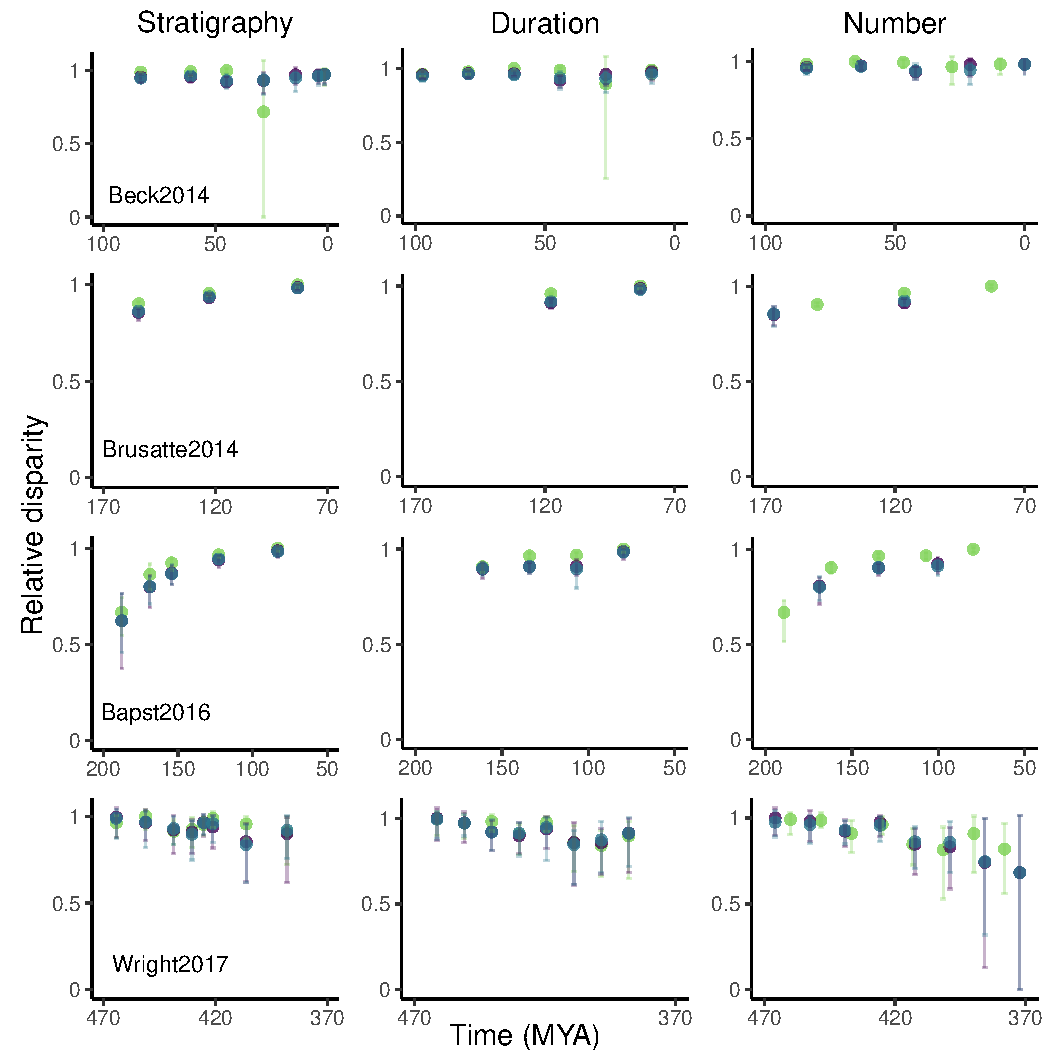
\includegraphics[width=1\linewidth, height=1\textheight, keepaspectratio]{figures/Figure2-fig-dtt-epoch-revision.pdf}
    \caption[Relative disparity-through-time.]
    {Relative disparity-through-time. Median bootstrapped disparities were calculated using time binning and time-slicing approaches. 
    Green points represent time binning methods, purple points are time-slices with a punctuated model of evolution (`proximity' method), and blue points are time-slices with a gradual model of evolution (`gradual splits' method).
    Relative disparities (median bootstrapped disparity divided by the maximum median bootstrapped disparity for a dataset and analysis method) are presented so they can be compared across datasets/methods. 
    Stratigraphy uses unequal time bins or non-equidistant time-slices, where the width of the bin, or the interval between slices, is equivalent to stratigraphic epochs. 
    Duration uses equal time bins or equidistant time-slices, where the width of the bin, or the interval between slices, is the average duration of stratigraphic epochs in the time frame of the dataset. 
    Number uses equal time bins or equidistant time-slices, where the number of bins, or the number of slices, is the average number of stratigraphic epochs in the time frame of the dataset. 
    In all cases, time bin disparities are plotted at the midpoint of the bin, and error bars represent the 95\% confidence intervals around the bootstrapped median disparity.
    The four dataset names are on the first plot for each dataset (see Table \ref{table:datasets} for details).
    Results for stratigraphic stages, and for other time-slicing methods, are in the Supporting Information Appendix S2: Figures A1-A2.}
    \label{figure:dtt1}
\end{figure}

\subsection{Testing for differences in the time sub-sampling methods}

\paragraph{Systematic differences in disparity-through-time.} 
There is no overall significant systematic difference among the disparities calculated using time bins and those calculated using the time-slicing methods (Table \ref{table:wilcox}, Supporting Information Appendix S2: Table A1).
Instead, the differences depend on the dataset and method in question.
For example, the \cite{brusatte2014gradual}, \cite{bapst2016topology} and \cite{wright2017bayesian} datasets, show significant differences when using bins versus time-slices defined by stratigraphy, but the \cite{beckancient2014} dataset appears robust to these different approaches.
Likewise, the \cite{beckancient2014}, \cite{brusatte2014gradual} and \cite{bapst2016topology} datasets have different disparities when the number of bins or slices is the average number of stratigraphic periods, but this is not seen in the \cite{wright2017bayesian} dataset.
Note that for epochs, we find fewer significant differences simply because the smaller numbers of bins and slices being compared means we have low power to detect a significant difference.

% Wilcoxon results table
%% latex table generated in R 3.4.2 by xtable 1.8-2 package
% Fri Dec  8 17:24:09 2017
\begin{table}[!htbp]
\caption{Results of paired Wilcoxon tests investigating whether disparities calculated using time bins are significantly different to those calculated using time-slices. Time-slices used either a  punctuated (‘proximity’ method) or gradual (‘gradual.split’ method) model of evolution. Stratigraphy uses unequal time bins or non-equidistant time-slices, where the width of the bin, or the interval between slices, is equivalent to stratigraphic ages or epochs. Duration uses equal time bins or equidistant time-slices, where the width of the bin, or the interval between slices, is the average duration of stratigraphic ages or epochs in the time frame of the dataset. Number uses equal time bins or equidistant time-slices, where the number of bins, or the number of slices, is the average number of stratigraphic ages or epochs in the time frame of the dataset. P-values were Bonferroni corrected. $***p < 0.001$. Results for other time-slicing methods are in the Supporting Information Appendix S2: Table A1.}
\centering
\begin{tabular}{lllccc}
  \hline
\textbf{Dataset} & \textbf{Period} & \textbf{Method} & \textbf{Stratigraphy} & \textbf{Duration} & \textbf{Number} \\ 
  \hline
  Beck2014 & Age & gradual.split & 111 & 115*** & 65*** \\ 
  Beck2014 & Age & proximity & 105 & 83 & 68*** \\ 
  Beck2014 & Epoch & gradual.split & 21 & 39 & 43*** \\ 
  Beck2014 & Epoch & proximity & 21 & 36 & 32 \\ 
  Brusatte2014 & Age & gradual.split & 28*** & 61*** & 52*** \\ 
  Brusatte2014 & Age & proximity & 27*** & 31 & 28*** \\ 
  Brusatte2014 & Epoch & gradual.split & 3 & 6 & 6 \\ 
  Brusatte2014 & Epoch & proximity & 0 & 5*** & 5 \\ 
  Bapst2016 & Age & gradual.split & 93 & 153 & 165 \\ 
  Bapst2016 & Age & proximity & 57*** & 47 & 75*** \\ 
  Bapst2016 & Epoch & gradual.split & 4 & 6 & 12 \\ 
  Bapst2016 & Epoch & proximity & 2 & 0*** & 8 \\ 
  Wright2017 & Age & gradual.split & 152*** & 155 & 116 \\ 
  Wright2017 & Age & proximity & 160*** & 175*** & 101 \\ 
  Wright2017 & Epoch & gradual.split & 28 & 29 & 21 \\ 
  Wright2017 & Epoch & proximity & 23 & 28 & 18 \\ 
   \hline
\end{tabular}

\label{table:wilcox} 
\end{table}
  

\paragraph{Disparity peaks.}
In the \cite{beckancient2014} and \cite{bapst2016topology} datasets, disparity peaks occur much at much older ages when time-slicing rather than time binning approaches are used (Fig. \ref{figure:peak1}; Supporting Information Appendix S2: Figs A3-A4).
This is also true for stratigraphic time bins in the \cite{wright2017bayesian} dataset, although when using equal time bins the peaks are later than the time-slicing methods, or very similar (Fig. \ref{figure:peak1}; Supporting Information Appendix S2: Figs A3-A4).
Across the three time binning methods, the \cite{brusatte2014gradual} dataset have similar disparity peaks whichever method is used, the \cite{wright2017bayesian} dataset only had variation in peaks when using un-equal time bins (stratigraphy) whereas in the \cite{bapst2016topology} and \cite{beckancient2014} datasets, stratigraphic (unequal) versus equally sized time bins make a large difference to where the disparity peak occurs (Fig. \ref{figure:peak1}; Supporting Information Appendix S2: Figs A3-A4).
Additionally, there seem to be low discrepancy within the time-slicing methods (gradual \textit{vs.} proximity) expect in \cite{beckancient2014} dataset where the gradual split model recovered disparity peaks at younger ages than the proximity model (Fig. \ref{figure:peak1}; Supporting Information Appendix S2: Figs A3-A4).

% Plots showing the differences
\begin{figure}[!htbp]
    \centering
    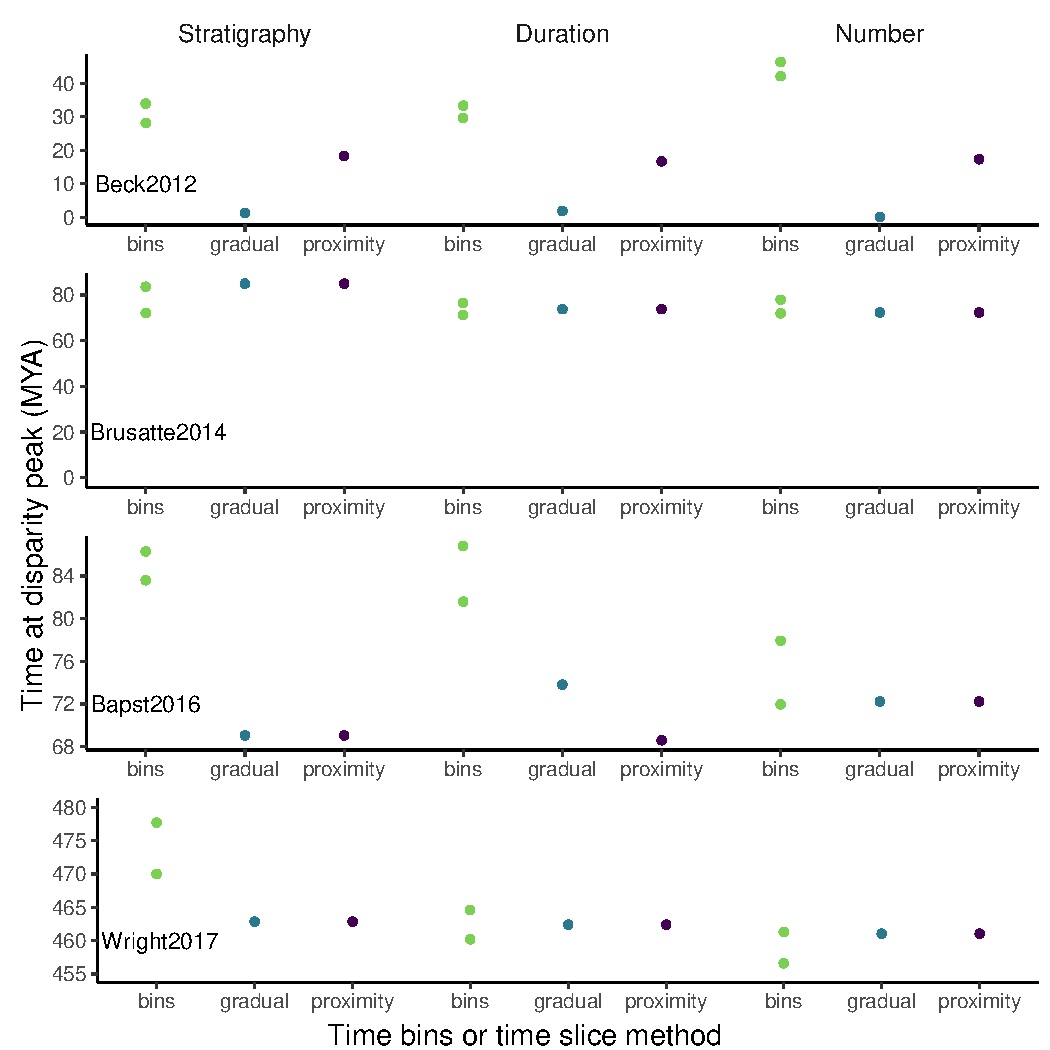
\includegraphics[width=1\linewidth, height=1\textheight, keepaspectratio]{figures/Figure3-fig-peaks-epoch-revision.pdf}
    \caption[Timing of peak disparity for four example datasets.]
    {Timing of peak disparity.
    Median bootstrapped disparities were calculated using time binning and time-slicing approaches. 
    Green points represent time binning methods, blue points are time-slices with a punctuated model of evolution (`proximity' method), and purple points are time-slices with a gradual model of evolution (`gradual splits' method). 
    Stratigraphy uses unequal time bins or non-equidistant time-slices, where the width of the bin, or the interval between slices, is equivalent to stratigraphic epochs. 
    Duration uses equal time bins or equidistant time-slices, where the width of the bin, or the interval between slices, is the average duration of stratigraphic epochs in the time frame of the dataset. 
    Number uses equal time bins or equidistant time-slices, where the number of bins, or the number of slices, is the average number of stratigraphic epochs in the time frame of the dataset. 
    For time bins the points indicate the maximum and minimum ages of the time bin within which peak disparities appeared.
    The four dataset names are on the first plot for each dataset (see Table \ref{table:datasets} for details).
    Results for stratigraphic stages, and for other time-slicing methods, are in the Supporting Information Appendix S2: Figures A3-A4.}
    \label{figure:peak1}
\end{figure}

\paragraph{Effects of mass extinction events.}
Mass extinction events influence disparity in both the \cite{beckancient2014} and \cite{wright2017bayesian} datasets (Fig. \ref{figure:extinction1}).
However, whether this change in disparity is significant or not depends on the method used to create time sub-samples (Fig. \ref{figure:extinction1}), and whether stages or epochs are used. 
In general, for the \cite{beckancient2014} dataset, time binning tended to give more significant results than time-slicing methods, but this was not the case for the \cite{wright2017bayesian} dataset.

% Big heat map table thing
\begin{figure}[!htbp]
    \centering
    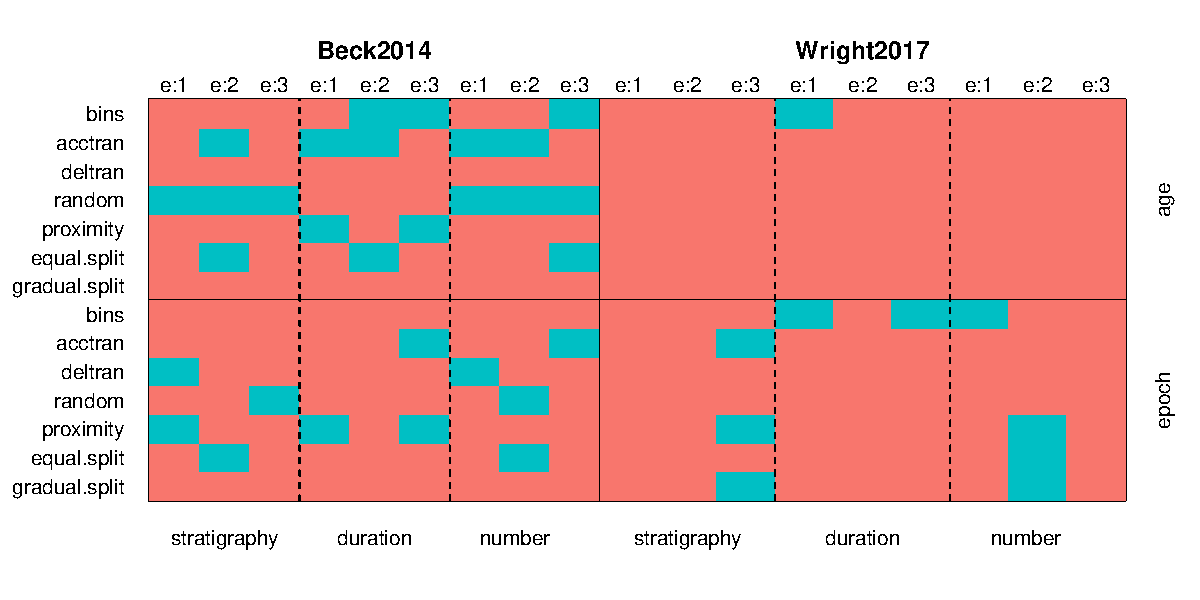
\includegraphics[width=1\linewidth, height=1\textheight, keepaspectratio]{figures/Figure4-fig-extinction-effect.pdf}
    \caption[Extinction example datasets.]
    {Effects of mass extinction events on disparity.
    Pink cells and blue cells indicate respectively a significant or non significant change in disparity before and after the mass extinction event (Cretaceous-Paleogene 66 MYA; \citealt{beckancient2014}; Ordovician-Silurian 455-430 MYA; \citealt{wright2017bayesian}).
    \textit{e:1}, \textit{e:2}, and \textit{e:3} denote whether the comparison was between the time bin or time-slice immediately after the mass extinction (\textit{e:1}), or the second (\textit{e:2}) or third (\textit{e:3}) bin/slice after the mass extinction to account for any lag effect.
    The top seven rows use stratigraphic stages and the bottom seven rows use stratigraphic epochs.
    Labels on the left hand side indicate whether time bins (``bins'') were used, or which of the six time-slicing methods was used.}
    \label{figure:extinction1}
\end{figure}

%Fig. or Figs
%Fig width 80mm single column
%110mm - 2/3 width
%166mm full page

\section{Discussion}
Disparity-through-time analyses are influenced by the choice of time sub-sampling method used to divide the taxa. 
While differences in the relative disparities calculated among time sub-sampling methods may not be of much biological importance, these changes can have important implications for the conclusions of downstream analyses. 
For example, using stratigraphic epochs as our reference time period, there are 21 potential methods for time sub-sampling our data (splitting by stratigraphy, number and duration, see methods, and using time bins or one of six time-slicing methods). 
Of these 21 methods, in 16 (76\%) we show that placental mammals \citep{beckancient2014} significantly increased in disparity in the time bin/slice immediately after the K-Pg mass extinction event, and in 20 (95\%) we show that crinoids \citep{wright2017bayesian} significantly decreased in disparity in the time bin/slice immediately after the O-S mass extinction event.
Given the high congruence (76\% and 95\%) of these results, one could argue that time-sub-sampling methods are not important. 
However, if we had chosen to investigate crinoid disparity only using time bins and splitting these so the number of time bins was equal to the number of epochs (number), we would have concluded that the O-S extinction had no effect on crinoid disparity. 
Likewise, the timing of peak disparity differs among methods. 
This is particularly evident when comparing stratigraphic time bins to time slicing methods, where for most of our datasets we see a much later time to peak disparity. 
This could have major implications for our understanding of how morphological diversity changes through time, for example in response to climate effects.
These results highlight the sensitivity of disparity-through-time analyses to the choice of time sub-sampling method. 
Fortunately this issue is easy to solve; either disparity-through-time analyses should use, and report results from, multiple time sub-sampling methods (as demonstrated here), or great care should be taken in determining the appropriate time sub-samples to answer the question of interest. 

Time-slicing has several advantages over time binning (using either equally or unequally sized bins) approaches.
First, it allows us to use as much of the information available to us, in the form of phylogenetic relationships and ancestral taxa, as possible. 
This increases our ability to investigate key biological questions, such as how do various drivers influence morphological diversity through time, and how do mass extinctions influence disparity \citep{Brusatte12092008,Foote29111996,friedmanexplosive2010}, both by increasing the statistical power of analyses and through the availability of data at key time points in the history of our groups.
Second, we are able to be more explicit about the mode of evolution in our clades; in time-slicing we can apply punctuated or gradual models of trait change rather than making an assumption of punctuated evolution.
This may be important, as gradual change is a common pattern of trait evolution in the fossil record \citep{Hunt20112007}.
Of course the method also has limitations.
The main one of these is a practical one; it requires a time-calibrated phylogeny.
Not all palaeontological datasets have phylogenies yet.
Another limitation is that the method, like most phylogeny based methods, depends on ancestral state estimations.
Care should be taken in interpreting these, as they are highly dependent on the data and models used for the estimations \citep{Slateretal2012,doi:10.1080/10635150801910451}.

\section{Conclusions}
The choice of time sub-sampling method can alter the conclusions we obtain from disparity-through-time studies. 
Time-slicing methods, with explicit models of evolution, provide an alternative to traditional time binning approaches.
Note that while we introduce the time-slicing methods here, and describe their advantages, we do not suggest time-slicing is necessarily the ``best'' method for time sub-sampling in all cases. 
As with all methods, the choice of methodology should be appropriate for the question and data at hand.
However, we do strongly recommend performing disparity-through-time analyses using a series of appropriate time sub-sampling methods, and comparing these, to ensure that results are not merely a consequence of the time sub-sampling method employed. 

\section{Data archiving statement}
Data for this study are available from \cite{dryad_n2g80,dryad_6hb7j,dryad_84t75,beckancient2014} but for ease of reproducibility can also be found on GitHub (\url{https://github.com/nhcooper123/time-slice/data}). % add proper link to zenodo
Supporting information can be found on Dryad at % Add Dryad link

\section{Supporting information}
Additional Supporting Information can be found in the online version of this article:\\
Appendix S1: Extra details of datasets. \\
Appendix S2: Additional figures. \\
Appendix S3: Additional tables.

\paragraph{Acknowledgments.}
  NC thanks Mark Sutton and Philip Mannion for the invitation to contribute to the `Evolutionary Modelling' symposium at The Palaeontological Association Annual Meeting 2017.
  TG acknowledges support from the Australian Discovery Project Grant number DP170103227 awarded to Vera Weisbecker.
  We thank Dave Bapst, Graeme Lloyd, April Wright and Davey Wright for assistance in gathering data for the analyses and/or discussions about the approach; and Steve Brusatte and one anonymous reviewer for helpful comments on the manuscript.

\section{References}

\bibliographystyle{palaeo} 
\bibliography{time-refs} 

\newpage
\section{Tables and Figures}

% Dataset details table
\begin{landscape}
% latex table generated in R 3.4.3 by xtable 1.8-2 package
% Wed Dec 20 13:12:18 2017
\begin{table}[!htbp]
\caption{Details of the datasets used in this study. Age ranges are root time to most recent tip taxon.} 
\centering
\begin{tabular}{lcccc}
  \hline
 & \textbf{Beck2014} & \textbf{Brusatte2014} & \textbf{Bapst2016} & \textbf{Wright2017} \\ 
  \hline
Group & mammals & theropods & theropods & crinoids \\ 
  \# taxa & 106 & 152 &  89 &  42 \\ 
  \# characters & 421 & 853 & 374 &  87 \\ 
  Age range (MYA) & 171.8 - 0 & 168.5 - 66 & 207.2 - 66 & 485.4 - 372.2 \\ 
  Mass extinction (MYA) & 66 (K-Pg) & NA & NA & 443 (O-S) \\ 
  Reference & \cite{beckancient2014} & \cite{brusatte2014gradual} & \cite{bapst2016topology} & \cite{wright2017bayesian} \\ 
  Data reference &  \cite{beckancient2014} & \cite{dryad_84t75} & \cite{dryad_n2g80} &  \cite{dryad_6hb7j} \\ 
   \hline
\end{tabular}
\label{table:datasets}  
\end{table}
 
\end{landscape}

% Wilcoxon results table
% latex table generated in R 3.4.2 by xtable 1.8-2 package
% Fri Dec  8 17:24:09 2017
\begin{table}[!htbp]
\caption{Results of paired Wilcoxon tests investigating whether disparities calculated using time bins are significantly different to those calculated using time-slices. Time-slices used either a  punctuated (‘proximity’ method) or gradual (‘gradual.split’ method) model of evolution. Stratigraphy uses unequal time bins or non-equidistant time-slices, where the width of the bin, or the interval between slices, is equivalent to stratigraphic ages or epochs. Duration uses equal time bins or equidistant time-slices, where the width of the bin, or the interval between slices, is the average duration of stratigraphic ages or epochs in the time frame of the dataset. Number uses equal time bins or equidistant time-slices, where the number of bins, or the number of slices, is the average number of stratigraphic ages or epochs in the time frame of the dataset. P-values were Bonferroni corrected. $***p < 0.001$. Results for other time-slicing methods are in the Supporting Information Appendix S2: Table A1.}
\centering
\begin{tabular}{lllccc}
  \hline
\textbf{Dataset} & \textbf{Period} & \textbf{Method} & \textbf{Stratigraphy} & \textbf{Duration} & \textbf{Number} \\ 
  \hline
  Beck2014 & Age & gradual.split & 111 & 115*** & 65*** \\ 
  Beck2014 & Age & proximity & 105 & 83 & 68*** \\ 
  Beck2014 & Epoch & gradual.split & 21 & 39 & 43*** \\ 
  Beck2014 & Epoch & proximity & 21 & 36 & 32 \\ 
  Brusatte2014 & Age & gradual.split & 28*** & 61*** & 52*** \\ 
  Brusatte2014 & Age & proximity & 27*** & 31 & 28*** \\ 
  Brusatte2014 & Epoch & gradual.split & 3 & 6 & 6 \\ 
  Brusatte2014 & Epoch & proximity & 0 & 5*** & 5 \\ 
  Bapst2016 & Age & gradual.split & 93 & 153 & 165 \\ 
  Bapst2016 & Age & proximity & 57*** & 47 & 75*** \\ 
  Bapst2016 & Epoch & gradual.split & 4 & 6 & 12 \\ 
  Bapst2016 & Epoch & proximity & 2 & 0*** & 8 \\ 
  Wright2017 & Age & gradual.split & 152*** & 155 & 116 \\ 
  Wright2017 & Age & proximity & 160*** & 175*** & 101 \\ 
  Wright2017 & Epoch & gradual.split & 28 & 29 & 21 \\ 
  Wright2017 & Epoch & proximity & 23 & 28 & 18 \\ 
   \hline
\end{tabular}

\label{table:wilcox} 
\end{table}
  

\end{document}